\subsection{Array Expansion}
In a CUDA kernel it is preferable that all memory is allocated before
starting it. That means that if we have a privatized variable or array in a loop
it is preferable that they are expanded with the outer dimensions such that we
can allocate the memory before executing the parallelized kernel.
In Figure \ref{fig:arr_exp} we can see a generalized array expansion from 1-dim
to 3-dim.

\begin{figure}[!ht]
    \centering
    \begin{minipage}{0.49\linewidth}
        \centering
		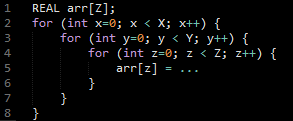
\includegraphics[scale=0.7]{input/figures/arr_exp1.png}
    \end{minipage}
    \begin{minipage}{0.49\linewidth}
        \centering
		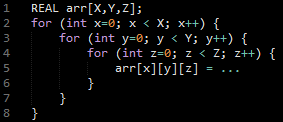
\includegraphics[scale=0.7]{input/figures/arr_exp2.png}
    \end{minipage}
\caption{Pseudo code array expanding an array into its two outer dimensions.\label{fig:arr_exp}}
\end{figure}

Such a transformation is always safe because each iteration writes and reads to its own
row of the array expanded array or variable. This should be given since before
the transformation the array or variable was private and hence unaffected by
other iterations.
We perform exactly such a expansion of the \emph{myResult} array. To do this we
also extract it from the PrivGlobs struct. \emph{myResult} is now a 3-dim
array, and we are able to compute \textbf{setPayoff} in a \emph{outer} loop as
we can see in Figure \ref{fig:new_myresult}.

\begin{figure}[!ht]
	\centering
		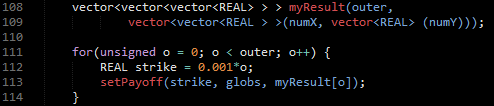
\includegraphics[scale=0.85]{input/figures/new_myResult.png}
		\caption{\label{fig:new_myresult}}
\end{figure}

Array expansion is a key concept we will utilize multiple times.

If we inline \emph{setPayoff} into the loop shown in Figure \ref{fig:new_myresult}
we can shorten the code and we are left with a loopnest that is fully
parallelizable as we can see in Figure \ref{fig:new_myresult2}.

\begin{figure}[!ht]
	\centering
		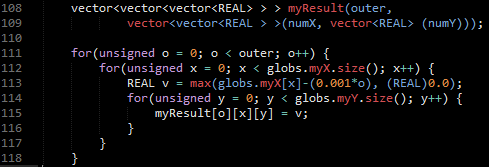
\includegraphics[scale=0.85]{input/figures/new_myResult2.png}
		\caption{\label{fig:new_myresult2}}
\end{figure}

It should be clear that there are no loop dependencies between each iteration
. We also note that the computed value is constant for each iteration of the
inner loop. Hence this computation can be extracted from the inner loop.
